\chapter{Enterprise Service Bus}
\label{cha:esb}
An Enterprise Service Bus (ESB) is a architectural pattern which describes a distributed computing architecture, where distributed services are connected to each other via the ESB. The ESB pattern if part of the Service Oriented Patterns (SOA).   
\\ \\
An ESB in the industry is mostly be taken as a third party platform, which provides features for implementing integrations with the Enterprise Integration-Patterns (EI). Enterprises use third party platforms like JBoss Fuse for implementing services, which integrate third party and internal systems. JBoss Fuse is based on the Enterprise Application-Platform (EAP), and bundles common frameworks used for integrations such as Camel, and provides implementation patterns for implementing the integration services.
\\ \\
The integration of internal as well as external services has become more important over time, especially with the upcoming of cloud solutions which provide PaaS. Common ESB platforms on the market usually define the ESB as a single application, which contains all integration services. But the need for flexibility and shorter response times drives enterprises to split up their teams and integrations. This leads to separated services, which are managed as microservices, which have their own life cycle. De-coupling of teams leads to de-coupling the services from their dependencies as well, where the dependencies need to provide a well defined and managed public API \cite{Camel2015, RedHatAgileIntegration2017, EIP}.

\section{The need for an Enterprise Service Bus}
\label{sec:esb-need-for-esb}
An ESB is needed by enterprises to provide integrations of their external service and internal services with other services, where the integration is meant to provide a business value for the enterprise. An integration of an external service could enhance the reach of a customer, who now could be able to consume an external partner service via the enterprise provided infrastructure. In the digital age it is normal to consume a digital service like Netflix, which runs a streaming service. Thus, integrations will become more over time, which will increase the number of services an enterprise will run for its integrations into other services and systems.

\section{Architecture}
\label{sec:esb-architecture}
Figure \vref{fig:esb-simple-architecture} illustrates the conceptional architecture of an ESB, which connects different services. A service can be either a producer service which gets accessed by clients, or a service can act as a consumer service, which acts as the client for a consumer service. The ESB is responsible for mediation, security, transformation, routing and service discovery. All these aspects are normally covered by an third party ESB platform, which runs the integration services. Such platforms provide all of the SOA/EI Patterns in form of a programming model \cite{EsbSoa2018, MediationESB2005}.

\begin{figure}[htbp]
	\centering
	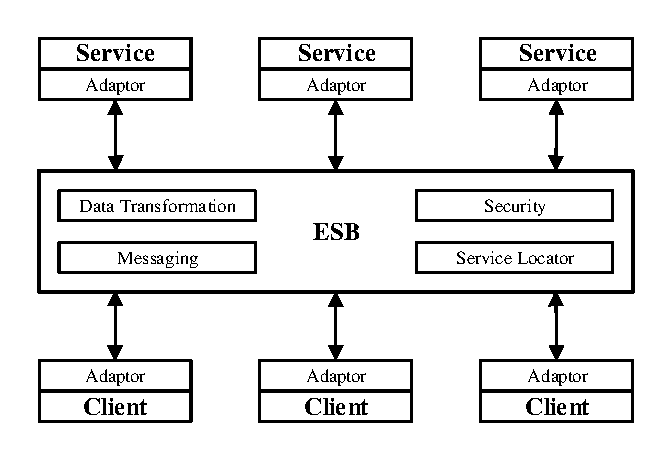
\includegraphics[scale=1]{images/esb-simple-architecture.pdf}
	\caption{Architecture of an ESB}
	\label{fig:esb-simple-architecture}
\end{figure} 

\begin{figure}[htbp]
	\centering
	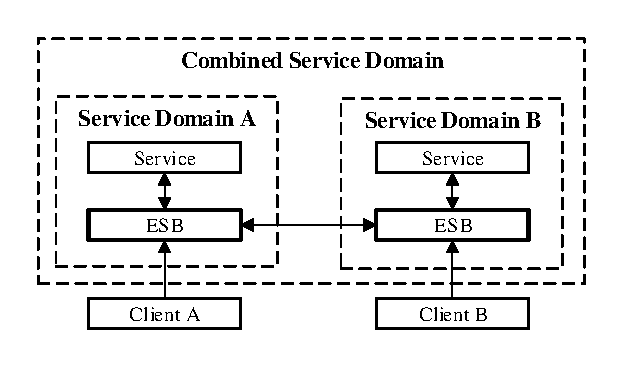
\includegraphics[scale=1]{images/esb-bidirectional-integration.pdf}
	\caption{Architecture of an bi-directional enterprise integration}
	\label{fig:esb-bidirectional-integration}
\end{figure} 

Figure \vref{fig:esb-bidirectional-integration} illustrates a bi-directional integration of services between two partner enterprises, where each integrated service is allowed to be consumed by the partner's customers, but only if the services is accessed via the partner's infrastructure. The ESB of the enterprises integrate the partner's provided service into their service domain, which can be accessed by their customers. For instance, an IP-TV provider can be integrated by an Internet Service-Provider (ISP), to provide Internet TV to their customers. 

\section{Enterprise Service Bus as Software}
\label{sec:esb-as-software}
An ESB is an architectural pattern for a distributed system, and has been implemented in software to provide an integration platform to developers, so that they can implemented integration services. Before the upcoming of the cloud, ESB implementations used existing platforms such as EAP, OSGI or Karaf for the service orchestration. In the case of EAP, the services are managed by an single process, whereby this single management process can be seen as a single point of failure for the whole ESB. Mostly the integration services are managed within a single application which represents the ESB, therefore the deployment of one integration service, leads to the deployment of the whole application. Figure \vref{fig:esb-software-architecture} illustrates the monolithic organization of the integration services within a single application.
\begin{figure}[htbp]
	\centering
	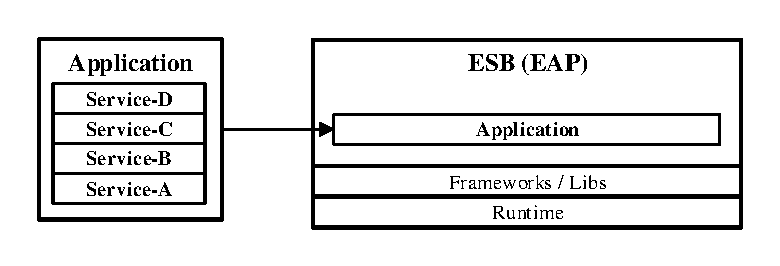
\includegraphics[scale=1]{images/esb-software-architecture.pdf}
	\caption{ESB application architecture with SOA}
	\label{fig:esb-software-architecture}
\end{figure} 

With the upcoming of cloud platforms such as PaaS, the cloud could take over the mediation, orchestration and security aspects of an ESB. The integration services are completely separated and de-coupled from each other, designed as microservices and their life cycle is managed by the cloud system. Additionally the ESB service are hosted in a cluster environment, which allows them to be distributed among multiple nodes, which increases fail over security. The new term for this kind of ESB is IPaaS, whereby the ESB is represented by an PaaS system such as Openshift \cite{iPaaSP12015, iPaaSP22015}.

\section{Enterprise Service Bus as Cloud}
\label{sec:esb-as-cloud}
With the upcoming and general availability of cloud platforms like PaaS, it was possible to move an ESB into the cloud, whereby the cloud platform takes over some aspects of the ESB platform such as mediation and service orchestration. A main problem of existing ESB implementations in enterprises is the fact that all of the integrations are managed within a single application, which represents the ESB. If the ESB is an cloud platform, the service have to be managed as microservices, which forces developers to separate their integration into separate code bases and to provide a proper designed and managed public API for their services.

\begin{figure}[htbp]
	\centering
	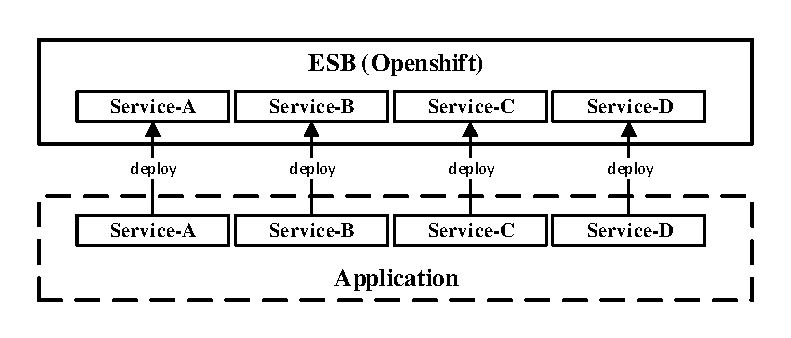
\includegraphics[scale=1]{images/esb-cloud-architecture.pdf}
	\caption{ESB application architecture with Microservices}
	\label{fig:esb-cloud-architecture}
\end{figure} 

As discussed in the introduction of this chapter, enterprises need to separate their integrations and teams, to be faster and more responsive to business changes. Therefore, the microservice architecture, which is necessary when the ESB is represented by an cloud platform, can help enterprises to separate their teams and integrations.  